%!TEX TS-program = xelatex
%!TEX encoding = UTF-8 Unicode

%\frame[plain]{ % When including a large figure or table, you don't want to have the bottom and the top of the slides.
%\frame[shrink]{ % If you want to include lots of text on a slide, use the shrink option.

% Explain why we did this research

\frame {
% add GNUNet logo and maybe some illustrative "surveillance-picture"
	\frametitle{Demo}
	 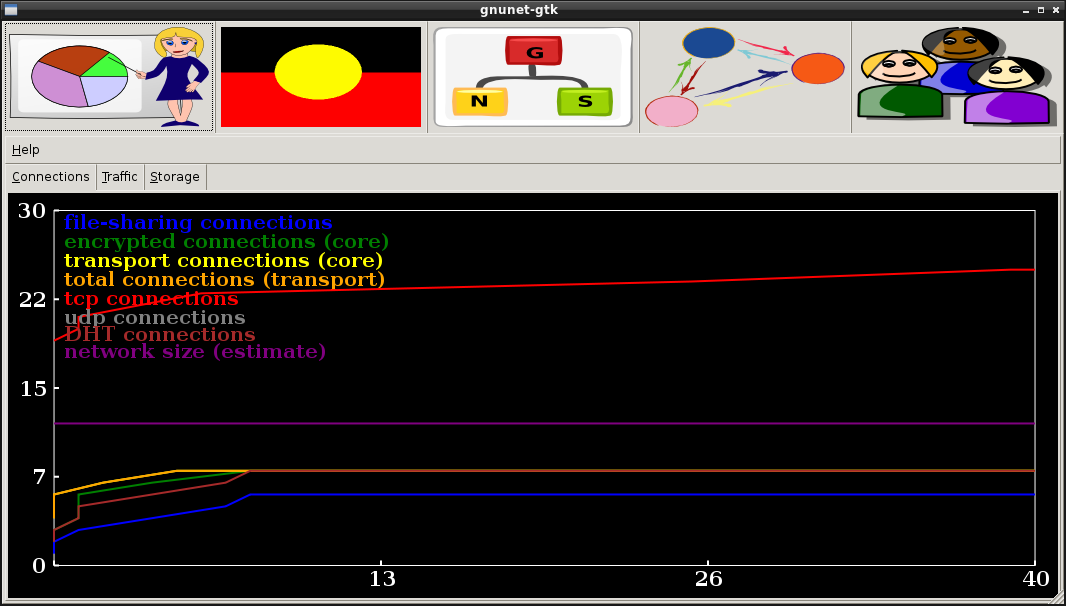
\includegraphics[width=1\textwidth]{frames/img/gnunet-gtk.png}

		\note{
			\begin{itemize}
				\item bla
			\end{itemize}
		}
}